% Final IEEE conference manuscript. Compile with pdfLaTeX in Overleaf.
\documentclass[conference]{IEEEtran}
\usepackage[utf8]{inputenc}
\usepackage[T1]{fontenc}
\usepackage{booktabs}
\usepackage{tabularx}
\usepackage{array}
\usepackage{graphicx}
\usepackage{amsmath}
\usepackage{amssymb}
\usepackage{cite}
\usepackage{url}
\usepackage[hidelinks]{hyperref}
\renewcommand{\arraystretch}{1.08}

\title{Version-Bound Readiness Reservations for Deadline-Aware Edge--Cloud Offloading under Artifact Eviction and Updates}
\author{\IEEEauthorblockN{Danish Atif (I22-1095) \qquad Salman Umar (I22-0908)}
\IEEEauthorblockA{Group G25, Section 7B, Cloud Computing\\
National University of Computer and Emerging Sciences, Pakistan}}

\begin{document}
\maketitle

\begin{abstract}
An edge scheduler can select a worker that appears ready, only to find at dispatch that the required artifact version has been evicted or replaced, or that its execution slot has been claimed. We study this dispatch-to-start readiness race with a deterministic discrete-event model of one constrained edge worker and a higher-latency cloud fallback. The proposed protocol atomically reserves an exact artifact version and one execution slot for a bounded, single-use token. We compare periodic advertisements, on-demand checking, artifact-only and slot-only ablations, and joint reservations across 24 configurations of dispatch delay, eviction rate, contention, and token lifetime; each configuration uses 30 shared seeds and 1,000 tasks per policy. In a representative high-stress condition (30~ms dispatch delay, 8 evictions/s, load coefficient 0.75, 50~ms token lifetime), joint reservation reaches 84.73\% deadline satisfaction versus 59.88\% for on-demand checking and 46.04\% for advertisements. It eliminates modeled dispatch-time readiness refusals while holding artifact state and occasionally wasting reserved slot time. These are simulation results, not a deployment-performance claim: hazards and costs are scenario parameters, and the model has one edge worker and no real container or control-plane implementation. The contribution is a reproducible, mechanism-focused characterization of the reliability--resource tradeoff.

\vspace{2pt}\noindent\textbf{Implementation and reproducibility artifact:}
\url{https://github.com/SalmannUmarr/edge-readiness-reservations}

\end{abstract}

\begin{IEEEkeywords}
edge--cloud offloading, serverless edge computing, readiness reservation,
artifact versioning, cache eviction, deadline-aware scheduling
\end{IEEEkeywords}

\section{Introduction}

Edge--cloud systems often choose an execution site from advertised artifact and capacity state. That observation can be stale before the request reaches the worker. During the resulting interval, a cache can evict or replace an exact function artifact, and competing work can occupy the observed slot. The scheduler then faces refusal, an initialization or retry path, or cloud fallback after part of the soft-deadline budget has already elapsed.

Existing systems make valuable but different contributions. AIHO addresses offloading and latency in serverless multi-edge-to-cloud systems \cite{li2025aiho}; AWL combines learned dispatch with warm-container-aware scheduling \cite{li2025awl}; and stale-load-aware offloading considers predictive information quality \cite{hamid2026staleness}. Serverledge provides implemented function offloading and migration across the edge--cloud continuum \cite{russo2024framework}. None of these results alone establishes a novelty claim for this work. Instead, this paper isolates a narrow question: what happens when both an exact artifact version and an execution slot can become unavailable between readiness observation and task start?

We evaluate a short-lived, version-bound readiness reservation. After atomically checking a requested artifact hash and a slot, the worker issues a single-use token tied to its epoch, the task, the hash, and an expiry. Until consumption, cancellation, or expiry, the token pins the artifact and holds the slot. The protocol does not promise survival across a crash, partition, or hard invalidation.

This paper makes three bounded contributions:
\begin{enumerate}
\item a precise dispatch-to-start model that separates artifact and slot hazards while preserving exact-version execution for every policy;
\item a five-policy controlled comparison, including artifact-only and slot-only ablations; and
\item seeded raw results, summaries, and tests supporting reproducibility of the simulation.
\end{enumerate}

\section{Related Work and Research Gap}

\subsection{Serverless offloading and warm artifacts}

Serverless edge scheduling must jointly consider communication delay, finite edge capacity, and whether a function is already warm. AIHO explicitly models local execution, peer-edge forwarding, cloud fallback, and cold start, then combines offloading, sorting, path selection, and function replacement \cite{li2025aiho}. AWL instead uses adaptive deep reinforcement learning for dispatch, a warm-aware queue discipline, and a container replacement rule; its Azure-derived evaluation shows that warm state and execution order affect SLO satisfaction \cite{li2025awl}. Experience-sharing DRL has also been used to coordinate distributed function offloading in resource-constrained serverless edges \cite{liu2023esdrl}. A broader survey classifies function-offloading approaches and identifies resource management, latency, and security as continuing challenges \cite{survey2024offloading}.

Implemented continuum frameworks strengthen the practical motivation. Serverledge supports decentralized horizontal and vertical offloading plus live function migration \cite{russo2024framework}. Its QoS-aware policies use service classes and distributed decisions to balance response time and edge capacity \cite{russo2024qos}. These works show that function location and initialization state matter, but their scheduling contracts do not preserve one exact artifact hash and one execution slot between observation and use.
Stateful serverless research additionally shows that exactly-once effects and
transactional workflows require explicit state and message guarantees rather than
stateless function invocation alone \cite{deheus2022transactions}; this motivates
our single-use token invariant without implying a full transaction protocol.

\subsection{Deadline, reliability, and stale state}

Deadline-aware edge scheduling is commonly formulated as an optimization over latency, energy, price, or SLO completion. Recent work combines martingale delay analysis, caching, and deep reinforcement learning \cite{dong2025delay}; other formulations optimize function pricing and offloading with PPO \cite{liu2025pricing}, application-dependent task graphs \cite{sun2021application}, or rapid edge--cloud placement under heterogeneous task requirements \cite{liu2024fast}. Surveys of fog scheduling emphasize the diversity of objectives and the difficulty of comparing evaluations across workloads \cite{hosseinzadeh2023survey}.

Uncertain state is directly relevant to our time-of-check-to-time-of-use problem. Hamid \emph{et al.} show that periodic load broadcasts can be stale and evaluate predictive load estimates \cite{hamid2026staleness}; uncertain processing cycles and intermittent connectivity similarly motivate robust offloading rather than decisions based on perfect observations \cite{deng2024uncertain}. Reliability-aware serverless deployment recognizes that dynamic function placement can fail under limited resources \cite{zhang2025reliability}. These approaches predict, optimize, or tolerate uncertain state. They do not create a bounded commitment that prevents the selected readiness state from changing before dispatch.

\subsection{Gap and positioning}

The closest studies account for warm containers, cache state, deadline risk, or stale measurements, but they treat an observation as information rather than a temporary resource grant. The gap is therefore not another latency predictor. It is the absence of a controlled evaluation of a joint, version-specific artifact pin and slot hold during the dispatch interval. Our work narrows the claim accordingly: we test whether protecting both readiness dimensions removes modeled dispatch refusals, quantify the resource cost, and separate the two effects with ablations. The official Komet artifact is used only for an independent released-trace verification and as provenance for the selected baseline; the formal bibliography below is limited to DOI-bearing journal articles as required by the course.

\section{Background and research question}

Komet is the selected baseline because its public artifact includes deterministic scheduling outputs suitable for a focused verification. We recalculate its \S8.1 trace-derived results from the released CSVs. Table~\ref{tab:komet} shows exact reproduction of migration counts and mean RTT agreement within 0.005~ms of values printed to two decimals. This is a verification of released traces, not a rerun of Komet's full distributed deployment.

\begin{table}[ht]
\centering
\caption{Komet \S8.1 released-trace verification.}
\label{tab:komet}
\small
\begin{tabular}{lrrr}
\toprule
Strategy & Paper RTT (ms) & Recalculated RTT (ms) & Migrations \\
\midrule
MinMax & 4.980 & 4.9849 & 16 \\
Komet 10\% & 4.990 & 4.9901 & 12 \\
Komet 25\% & 5.220 & 5.2177 & 9 \\
Komet 1 ms & 5.040 & 5.0373 & 12 \\
\bottomrule
\end{tabular}
\end{table}

Our research question is: \emph{Can short-lived, version-bound readiness reservations improve deadline satisfaction under artifact eviction and updates, while preserving correct-version execution and acceptable worker utilization, compared with readiness advertisements and on-demand readiness checks without reservations?}

We test four expectations: (i) a valid joint reservation reduces dispatch-time refusal relative to on-demand checking; (ii) fewer refusals improve deadline satisfaction where fallback is costly; (iii) single-resource reservations have intermediate outcomes when both hazards are active; and (iv) a token lifetime shorter than dispatch delay cannot preserve readiness.

\section{Protocol and model}

Figure~\ref{fig:architecture} summarizes the control path. The scheduler observes
task metadata and worker readiness, obtains either an unprotected readiness answer
or a reservation token, and dispatches after a control-plane delay. The cloud path
is deliberately common to every policy so that differences arise from edge
readiness rather than a privileged fallback rule.

\begin{figure*}[t]
\centering
\setlength{\fboxsep}{6pt}
\fbox{\parbox{0.16\textwidth}{\centering\textbf{Task source}\\version hash\\arrival, deadline}}
\hspace{3pt}$\longrightarrow$
\fbox{\parbox{0.21\textwidth}{\centering\textbf{Scheduler}\\estimate completion\\select policy and target}}
\hspace{3pt}$\longleftrightarrow$
\fbox{\parbox{0.23\textwidth}{\centering\textbf{Edge worker}\\artifact cache + epoch\\single execution slot}}
\hspace{3pt}$\dashrightarrow$
\fbox{\parbox{0.17\textwidth}{\centering\textbf{Cloud fallback}\\reliable but higher latency}}
\\[5pt]
\fbox{\parbox{0.73\textwidth}{\centering Reservation response binds
$(\text{worker epoch},\text{task ID},\text{artifact hash},\text{nonce},\text{expiry})$;
dispatch atomically consumes it once or receives a categorized refusal.}}
\caption{Logical workflow of version-bound readiness reservation and the common fallback path.}
\label{fig:architecture}
\end{figure*}

\subsection{Reservation protocol}

The scheduler selects a candidate using a common completion-time estimator. It asks the worker to atomically check the requested version and a free execution slot. A successful worker returns a token containing the worker epoch, task identifier, exact artifact hash, reservation identifier, and expiry. The scheduler dispatches only while the token is valid and the remaining deadline budget permits. The worker consumes a token at most once after validating all fields. Cancellation or expiry releases the pin and slot; a restart invalidates tokens by changing the worker epoch. A mismatch is a refusal, never execution of a substitute local version.

The protocol is deliberately conditional. It does not provide a hard real-time guarantee, distributed crash recovery, token authentication, or clock synchronization across workers. A networked prototype would need unguessable or signed tokens, persistent replay protection where required, and measured control-plane margins.

\subsection{Simulator}

The discrete-event simulator has one scheduler, one single-slot edge worker, and a reliable but higher-latency cloud fallback. Each task has an arrival time, exact version, absolute soft deadline, edge RTT, and runtime. Between selection and dispatch, independent stochastic events may evict or replace the artifact or claim the slot. Failed edge starts fall back to cloud after a fixed retry penalty. All policies enforce the same exact-version rule, placement estimator, deadlines, edge/cloud costs, and fallback logic.

The comparison policies are:
\begin{enumerate}
\item \textbf{Advertisement}: select from a periodic readiness snapshot.
\item \textbf{On-demand}: query current readiness but hold neither resource.
\item \textbf{Artifact-only}: pin the requested version but not the slot.
\item \textbf{Slot-only}: hold the slot but not the artifact version.
\item \textbf{Joint reservation}: atomically pin the version and hold the slot.
\end{enumerate}

The model does not represent real cache eviction, container image transfer, multiple worker queues, correlated failures, satellite dynamics, authentication overhead, or energy and monetary costs. It therefore tests internal mechanism behavior rather than production-cloud superiority.

\subsection{Decision rule and reservation cost}

For task $i$ and candidate $w$, the scheduler admits an edge dispatch only if the
estimated completion time
\begin{equation}
 \widehat{C}_{i,w}=a_i+d_{i,w}+q_{i,w}+x_{i,w}
 \label{eq:completion}
\end{equation}
does not exceed absolute deadline $D_i$. Here $a_i$ is arrival time, $d_{i,w}$
is the decision-to-start communication delay, $q_{i,w}$ is modeled queue or
readiness delay, and $x_{i,w}$ is execution time. A failed edge start adds a
fixed retry penalty before the same cloud fallback used by every policy.

Let token $r$ have issue time $t_r$, expiry $e_r$, artifact size $B_r$, slot
indicator $s_r$, and consumption or release time $u_r$. The simulator accounts
for artifact holding as
\begin{equation}
 H_B=\sum_r B_r\max(0,\min(u_r,e_r)-t_r)
\end{equation}
and slot holding analogously with $B_r$ replaced by $s_r$. Unused slot time is
the held interval for tokens cancelled or expired without execution. These terms
make explicit that refusal avoidance consumes finite resources.

The primary outcome for a configuration $c$ is
\begin{equation}
 S_c=\frac{\sum_i \mathbf{1}[C_i\leq D_i]}{N_c},
\end{equation}
where $N_c$ includes every submitted task, including cancellations and terminal
failures. Keeping those cases in the denominator prevents a policy from appearing
better merely because unsuccessful work disappears from analysis. Readiness
refusal is counted only when a selected edge start cannot acquire the exact
artifact version or slot. Cloud fallback is recorded independently, because a task
can fall back for admission reasons without a dispatch-time refusal. Correct-version
execution is checked at every successful edge start.

The reservation transaction proceeds in four steps. First, the scheduler sends
the task identity, exact hash, required resources, and requested expiry. Second,
the worker checks epoch-local token state, artifact presence, and slot availability
under one logical lock. Third, if both resources are available, the worker creates
the nonce, pins the hash, marks the slot held, and returns the bound token; otherwise
it returns a categorized refusal without partial state. Fourth, dispatch validates
all fields and consumes the token atomically. Cancellation and expiry use the same
release operation so that a partially released reservation cannot survive.

This transaction is intentionally narrower than a distributed lock or general
lease service. The worker does not promise recovery of a reservation after restart,
and the scheduler cannot extend a token silently. A longer lifetime requires a new
admission decision because capacity may have changed. This bounded behavior limits
failure-related blocking and makes resource consumption visible in the measured
holding metrics.

\subsection{Safety invariants}

A token is valid only when worker epoch, task identity, artifact hash, nonce, and
expiry all match. Consumption is atomic and single-use. A version mismatch is a
refusal rather than permission to run a substitute version. Pins and slots end on
consumption, explicit cancellation, or expiry, while a worker restart changes the
epoch and invalidates outstanding tokens. The simulator tests exact-version
execution, valid-lifetime protection, expiry behavior, and deterministic traces.

\section{Experimental method}

The frozen matrix varies dispatch delay (10 or 30~ms), eviction rate (2 or 8 events/s), competing-load coefficient (0.35 or 0.75), and reservation lifetime (20, 50, or 100~ms), yielding 24 cells. Each policy is run for 30 independent seeds of 1,000 tasks. Within a seed, policies receive the same generated tasks and random variates, enabling paired comparisons. Defaults include 18 arrivals/s, 4 replacement events/s, 24~ms edge runtime, 42~ms cloud runtime, 62~ms cloud RTT, 50~ms advertisement interval, 12~ms retry penalty, 128~MB artifact size, and 2\% cancellations. Deadlines are uniformly 92--142~ms after arrival and edge RTT is uniformly 9--21~ms.

The primary metric is deadline satisfaction: completed-by-deadline tasks divided by all submitted tasks. Secondary metrics are dispatch-time refusal rate, fallback rate, mean and p95 latency, control messages, pinned MB-seconds, and unused reserved slot-seconds. Reported confidence intervals are 95\% normal intervals across the 30 seed-level observations ($1.96s/\sqrt{30}$). The raw rows remain available for paired analysis; we do not infer statistical significance solely from confidence-interval overlap.

\subsection{Factor selection and fairness controls}

The matrix is a mechanism-focused factorial design. Two dispatch delays determine
whether a 20~ms token is adequate or expires before use. Two eviction rates create
moderate and stressed artifact conditions. Two competing-load coefficients expose
the slot dimension, while three token lifetimes test under-coverage, sufficient
coverage, and over-provisioned lifetime. The resulting $2\times2\times2\times3$
design contains 24 cells. Thirty independent seeds balance interval stability with
fast reproducibility on ordinary hardware.

Five controls keep the comparison interpretable. First, every policy receives the
same task objects and random hazard variates for a seed. Second, exact-version
validation is mandatory for every policy; no baseline gains latency by executing a
wrong version. Third, cloud runtime, RTT, retry penalty, and deadline feasibility
logic are shared. Fourth, each policy sees the same edge runtime and artifact size.
Fifth, cancellations count against submitted work and reservation waste is retained.
Only the readiness-information and holding semantics differ.

The advertisement baseline represents low-control-overhead discovery from a
periodically refreshed snapshot. On-demand represents a fresh check without a
commitment. These two policies bound the value of fresher information alone. The
artifact-only and slot-only policies are causal ablations rather than intended
deployments: each protects one possible source of invalidated readiness. The joint
policy tests the proposed atomic protection. This progression prevents a result
from being attributed vaguely to ``reservation'' when only one resource matters.

\subsection{Random variables and event order}

Task inter-arrivals are exponentially distributed at the frozen arrival rate.
Deadlines and edge RTTs use the bounded uniform distributions in
Table~\ref{tab:config}. Eviction and replacement processes represent loss of the
requested artifact or substitution by a different version. Competing load can
claim the single edge slot during the dispatch interval. Cancellations occur after
a reservation decision and therefore reveal unused holding cost. All random draws
are derived from a seed-specific generator and materialized before policy replay.

Event ordering is deterministic when timestamps match. Expiry is evaluated before
token consumption at the same timestamp, so a token is valid strictly within its
declared lifetime. Artifact mismatch and slot unavailability are recorded
separately; a start affected by both contributes once to total readiness refusal.
The cloud completion time includes retry cost only after a failed selected edge
start. These rules are fixed across the matrix and tested for deterministic replay.

\begin{table}[t]
\centering
\caption{Frozen experimental factors and defaults.}
\label{tab:config}
\footnotesize
\begin{tabular}{ll}
\toprule
Parameter & Value(s) \\
\midrule
Dispatch delay & 10, 30 ms \\
Eviction rate & 2, 8 events/s \\
Competing-load coefficient & 0.35, 0.75 \\
Reservation lifetime & 20, 50, 100 ms \\
Independent seeds & 1--30 \\
Tasks per policy/cell & 1,000 \\
Arrival rate & 18 tasks/s \\
Replacement rate & 4 events/s \\
Edge/cloud runtime & 24/42 ms \\
Cloud RTT; retry penalty & 62 ms; 12 ms \\
Deadline offset & Uniform 92--142 ms \\
Cancellation probability & 0.02 \\
\bottomrule
\end{tabular}
\end{table}

\section{Implementation and Reproducibility}

The implementation is a standard-library Python discrete-event simulator. An
immutable configuration object records every frozen factor. A workload generator
creates task arrivals, version requests, deadlines, RTTs, eviction/replacement
events, contention events, and cancellations. Each seed generates this trace once;
all five policies replay the same task and hazard variates, which reduces
between-policy noise without sharing mutable policy state.

The policy layer implements a common interface and common placement estimator.
Advertisement reads a cached snapshot refreshed at a fixed interval. On-demand
checks the current cache and slot but releases both before dispatch. Artifact-only
and slot-only preserve exactly one readiness dimension. Joint reservation performs
the check and both holds as one state transition. The execution layer categorizes
artifact and slot refusals, applies cloud fallback, and records terminal outcomes.
The metrics layer writes one CSV row per policy and seed, then aggregates by
configuration with means and 95\% confidence intervals.

The artifact also contains a separate script that recalculates Komet's released
Section~8.1 scheduling CSVs. All four published migration counts match exactly and
the largest mean-RTT difference is 0.0049~ms, consistent with rounding to two
decimal places. This check validates our aggregation path against released data;
it is not presented as a rerun of Komet's original distributed deployment.

Reproduction requires Python~3 and no third-party runtime dependencies. From the
repository root, the complete verification is:
\begin{verbatim}
python3 scripts/reproduce_komet.py
python3 -m unittest discover -s tests -v
python3 scripts/run_experiments.py
\end{verbatim}
The final command deterministically writes 3,600 seed-level rows and 120 aggregate
rows. The repository retains source, tests, baseline CSVs, raw outputs, summaries,
and this manuscript so an evaluator can demonstrate every reported number.

\section{Results}

\subsection{Aggregate matrix view}

Table~\ref{tab:overall} gives an unweighted descriptive mean across the 24 retained
cells. It is not a substitute for factor-specific analysis: the table deliberately
mixes token lifetimes that do and do not cover dispatch. It is useful as a compact
check that the representative stress condition is not the only cell in which the
policy ordering appears. Across the full matrix, joint reservation has the highest
deadline satisfaction and lowest mean latency and refusal rate. Its residual
3.34\% refusal is explained by cells where the 20~ms lifetime expires before a
30~ms dispatch.

\begin{table*}[t]
\centering
\caption{Unweighted descriptive mean over all 24 configuration cells.}
\label{tab:overall}
\small
\begin{tabular}{lrrrrr}
\toprule
Policy & Deadline met (\%) & Refusal (\%) & Fallback (\%) & Mean latency (ms) & Messages/run \\
\midrule
Advertisement & 60.70 & 34.78 & 69.81 & 101.66 & 523 \\
On-demand & 73.04 & 14.16 & 70.20 & 95.23 & 2,523 \\
Artifact-only & 76.32 & 9.94 & 67.82 & 92.73 & 3,365 \\
Slot-only & 78.00 & 8.67 & 64.10 & 90.74 & 3,414 \\
Joint reservation & \textbf{82.15} & \textbf{3.34} & \textbf{61.38} & \textbf{87.67} & 3,362 \\
\bottomrule
\end{tabular}
\end{table*}

\subsection{Representative stress condition}

Table~\ref{tab:stress} reports the most demanding retained condition: 30~ms dispatch delay, 8 evictions/s, competing-load coefficient 0.75, and 50~ms lifetime. A 50~ms lifetime covers the 30~ms dispatch interval. Joint reservation has no modeled readiness refusals and achieves the highest deadline satisfaction. Relative to on-demand, the absolute improvement is 24.85 percentage points; relative to advertisement, it is 38.69 points. All policies record zero invalid-version executions because exact-version rejection is enforced uniformly.

\begin{table*}[ht]
\centering
\caption{Mean outcomes in the representative stress condition; $\pm$ is the 95\% interval across 30 seeds.}
\label{tab:stress}
\small
\begin{tabularx}{\textwidth}{lrrrrr}
\toprule
Policy & Deadline satisfaction & Refusal rate & Mean latency (ms) & p95 (ms) & Messages/run \\
\midrule
Advertisement & 46.04\% $\pm$ 0.57 & 43.51\% & 117.03 & 146 & 523 \\
On-demand & 59.88\% $\pm$ 0.61 & 25.69\% & 109.39 & 146 & 2,523 \\
Artifact-only & 67.47\% $\pm$ 0.54 & 17.36\% & 104.15 & 146 & 3,294 \\
Slot-only & 72.78\% $\pm$ 0.57 & 13.59\% & 98.88 & 146 & 3,429 \\
Joint reservation & \textbf{84.73\% $\pm$ 0.46} & \textbf{0.00\%} & \textbf{90.81} & \textbf{104} & 3,285 \\
\bottomrule
\end{tabularx}
\end{table*}

\begin{figure}[t]
\centering
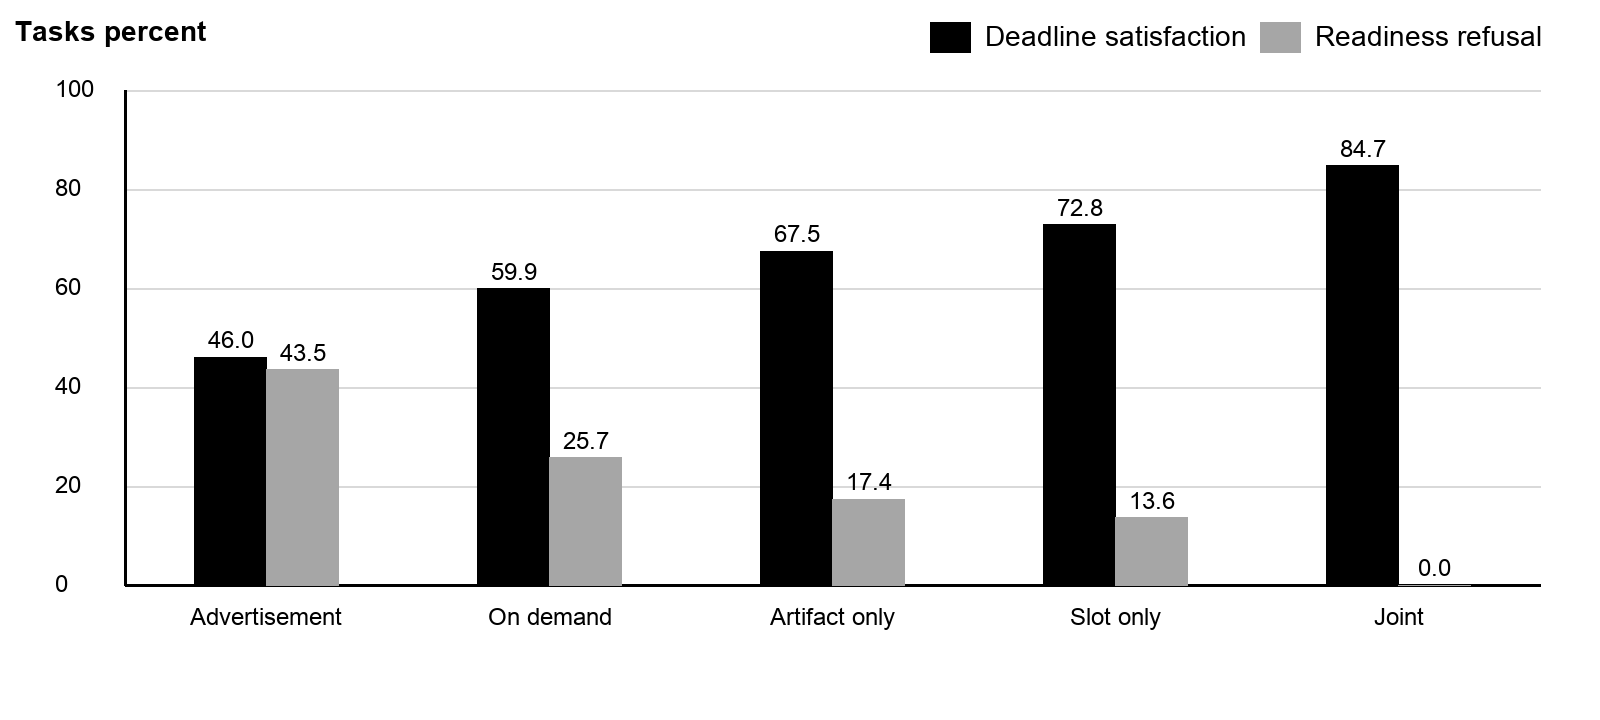
\includegraphics[width=\columnwidth]{figures/policy_comparison.png}
\caption{Deadline satisfaction and readiness refusal in the representative stress condition. Error bars are 95\% confidence intervals across 30 seeds.}
\label{fig:policycomparison}
\end{figure}

The ablations support the mechanism interpretation without proving generality. Artifact-only reservation leaves slot contention exposed; slot-only reservation leaves eviction and replacement exposed. Slot-only is stronger in this cell because the configured competing-slot hazard is more influential than the modeled artifact hazard. That result should not be generalized to other systems or workloads.

\subsection{Lifetime boundary and resource cost}

At 30~ms dispatch delay, a 20~ms lifetime expires before dispatch. It therefore cannot protect either resource for the full gap, and readiness refusals remain possible. At 50 and 100~ms, the token covers dispatch and joint reservation removes the modeled race; the longer lifetime has no further readiness benefit in this model.

The benefit is not free. In the representative stress condition, joint reservation pins approximately 1,464~MB-seconds of artifact state per 1,000-task seed and wastes about 0.233~seconds of reserved slot time because of cancellation. It sends more messages than advertisement or on-demand checking. These costs make token-duration selection a resource-allocation decision: the appropriate lifetime is bounded just above measured control-plane delay, not maximized.

Table~\ref{tab:ttl} isolates the lifetime boundary in the same stress setting. At
20~ms, the joint token expires before the 30~ms dispatch and consequently collapses
to the on-demand outcome: 59.88\% deadline satisfaction and 25.69\% refusal. At
50~ms, both protected resources survive through dispatch, deadline satisfaction
rises to 84.73\%, and modeled refusal becomes zero. Increasing lifetime to 100~ms
does not improve these outcomes because successful tokens are consumed at dispatch;
the retained mean holding cost is consequently unchanged in this model. A real
system with queueing before consumption could produce a different cost curve.

\begin{table}[t]
\centering
\caption{Joint-reservation lifetime in the stress condition.}
\label{tab:ttl}
\footnotesize
\begin{tabular}{rrrrr}
\toprule
TTL & Deadline & Refusal & Unused slot & Pinned \\
(ms) & (\%) & (\%) & (s) & (MB-s) \\
\midrule
20 & 59.88 & 25.69 & 0.181 & 1,079.9 \\
50 & 84.73 & 0.00 & 0.233 & 1,464.2 \\
100 & 84.73 & 0.00 & 0.233 & 1,464.2 \\
\bottomrule
\end{tabular}
\end{table}

\subsection{Cross-scenario interpretation}

The retained matrix contains both low- and high-churn settings rather than only the
representative cell plotted in Fig.~\ref{fig:policycomparison}. Advertisement is
most exposed because its snapshot can already be stale at selection. On-demand
removes pre-decision staleness but leaves the dispatch interval unprotected. The
two single-resource ablations identify which hazard dominates a cell: slot-only is
stronger when contention dominates, whereas artifact-only gains relative value as
eviction and replacement pressure increase. Joint reservation eliminates modeled
dispatch refusals only when its lifetime covers the dispatch delay; it does not
remove cancellation, deadline infeasibility, or cloud latency.

The confidence intervals describe variation across independent seeds, not across
real deployments. Common random numbers enable direct paired follow-up analysis,
but the present paper avoids claiming population-level significance from interval
overlap alone. Most importantly, all policies produce zero invalid-version
executions. The deadline gain is therefore not purchased by relaxing semantic
correctness.

\section{Discussion}

The results support the narrow causal explanation built into the simulator: if a token atomically protects the two resources that otherwise change between check and use, there is no modeled dispatch-time refusal while the token remains valid. The gain in deadline satisfaction follows because cloud fallback has a larger latency penalty. This is not evidence that a reservation will improve every edge deployment, nor that the simulated hazard rates match a real platform.

The comparison is deliberately fair in one important sense: no baseline can execute the wrong artifact version. A design that allowed stale-version execution could superficially improve latency while violating the task contract. Correct-version execution is therefore treated as a safety requirement, not a competing optimization target.

\subsection{Operational implications}

The mechanism is appropriate only when readiness can change materially during the
control interval and fallback consumes deadline budget. A deployment should measure
decision-to-start delay and set a bounded lifetime slightly above a high percentile
of that distribution. A larger lifetime does not improve already-covered dispatches
but increases exposure to idle resource holding. Admission control should cap the
number or fraction of reserved slots and pinned bytes, while the scheduler should
avoid issuing a token when the remaining deadline cannot accommodate dispatch and
execution.

The token fields are also part of the failure model. Worker epochs prevent a token
issued before restart from authorizing execution afterward. Nonces and atomic
consumption prevent replay within an epoch. Production workers would additionally
need authenticated transport, unguessable or signed tokens, monotonic local expiry,
bounded clock assumptions, and idempotent result handling across retries. These
controls are design requirements, not features validated by this simulator.

\subsection{Threats to validity}

\textit{Internal validity:} the joint policy protects precisely the hazards injected
by the model, so zero refusal with a valid token is partly structural. The ablations,
expired-token test, and identical random traces help isolate this mechanism but do
not remove modeling bias. \textit{Construct validity:} hazard rates and the competing
load coefficient are scenario controls rather than field measurements. Control
messages approximate protocol effort but do not measure CPU, serialization, or
cryptographic cost. \textit{External validity:} the model uses one edge worker and
one slot, independent hazards, perfect local time, and reliable cloud fallback. It
does not model correlated cache pressure, network partitions, energy, monetary cost,
or heterogeneous multi-worker queues. \textit{Reproducibility validity:} fixed seeds,
raw rows, scripts, and tests permit exact reruns, but Python-version and platform
metadata should still be recorded in a public release. The Komet verification
corroborates released-trace aggregation only; it does not validate our protocol.

\section{Reproducibility and next validation}

The artifact contains the simulator, fixed seed matrix, raw per-run results, summaries, baseline aggregation script, and unit tests. The following commands reproduce the retained outputs:

\begin{verbatim}
python3 scripts/reproduce_komet.py
python3 -m unittest discover -s tests -v
python3 scripts/run_experiments.py
\end{verbatim}

The next empirical phase should implement two constrained edge workers and one cloud-role worker in containers, measure cache initialization, execution, and control-plane costs, then freeze a calibrated configuration before confirmatory runs. It should add worker epochs and unguessable or signed tokens, test restart/cancellation/replay behavior, and report all terminal failure categories. Until that work is completed, the present contribution must be described as a reproducible simulation study.

\section{Conclusion}

Version-bound readiness reservations address a specific time-of-check-to-time-of-use race: a chosen worker can lose either the requested artifact version or a free execution slot before dispatch. In a seeded single-worker simulation, joint reservations eliminate the modeled readiness refusal when their lifetime covers dispatch and improve deadline satisfaction in high-churn, high-contention conditions. The improvement requires more control work and resource holding, and the model's constraints prohibit a deployment claim. The principal result is a transparent basis for a calibrated container testbed, not a universal scheduling guarantee.

\begin{thebibliography}{99}
\bibitem{li2025aiho} X. Li, L. Chen, Z. Yuan, and G. Liu, ``AIHO: Enhancing task offloading and reducing latency in serverless multi-edge-to-cloud systems,'' \emph{Future Generation Computer Systems}, vol. 165, art. 107607, 2025, doi: 10.1016/j.future.2024.107607.

\bibitem{li2025awl} M. Li, F. Xu, Y. Wu, J. Zhang, W. Xu, and Y. Wu, ``Real-time task dispatching and scheduling in serverless edge computing,'' \emph{Ad Hoc Networks}, vol. 174, art. 103854, 2025, doi: 10.1016/j.adhoc.2025.103854.

\bibitem{hamid2026staleness} S. A. Hamid, Y. Boujelben, and F. Zarai, ``Exploiting and mitigating staleness in distributed edge offloading via predictive load awareness,'' \emph{Network}, vol. 6, no. 3, art. 69, 2026, doi: 10.3390/network6030069.

\bibitem{russo2024framework} G. Russo Russo, V. Cardellini, and F. Lo Presti, ``A framework for offloading and migration of serverless functions in the Edge--Cloud Continuum,'' \emph{Pervasive and Mobile Computing}, vol. 100, art. 101915, 2024, doi: 10.1016/j.pmcj.2024.101915.

\bibitem{liu2023esdrl} X. Yao, N. Chen, X. Yuan, and P. Ou, ``Performance optimization of serverless edge computing function offloading based on deep reinforcement learning,'' \emph{Future Generation Computer Systems}, vol. 139, pp. 74--86, 2023, doi: 10.1016/j.future.2022.09.009.

\bibitem{survey2024offloading} M. Ghorbian and M. Ghobaei-Arani, ``Function offloading approaches in serverless computing: A survey,'' \emph{Computers \& Electrical Engineering}, vol. 120, art. 109832, 2024, doi: 10.1016/j.compeleceng.2024.109832.

\bibitem{russo2024qos} G. Russo Russo, D. Ferrarelli, D. Pasquali, V. Cardellini, and F. Lo Presti, ``QoS-aware offloading policies for serverless functions in the Cloud-to-Edge continuum,'' \emph{Future Generation Computer Systems}, vol. 156, pp. 1--15, 2024, doi: 10.1016/j.future.2024.02.019.

\bibitem{deheus2022transactions} M. de Heus, K. Psarakis, M. Fragkoulis, and A. Katsifodimos, ``Transactions across serverless functions leveraging stateful dataflows,'' \emph{Information Systems}, vol. 108, art. 102015, 2022, doi: 10.1016/j.is.2022.102015.

\bibitem{dong2025delay} C. Dong, W. Li, Z. Zhou, X. Chen, Z. Tian, and W. Wen, ``Delay-sensitive task offloading with edge caching through martingale-based deep reinforcement learning,'' \emph{IEEE Transactions on Mobile Computing}, vol. 24, no. 7, pp. 6225--6242, 2025, doi: 10.1109/TMC.2025.3540413.

\bibitem{liu2025pricing} S. Liu, L. Pan, and S. Liu, ``A profit-effective function service pricing approach for serverless edge computing function offloading,'' \emph{Journal of Network and Computer Applications}, vol. 244, art. 104338, 2025, doi: 10.1016/j.jnca.2025.104338.

\bibitem{sun2021application} M. Sun, T. Bao, D. Xie, H. Lv, and G. Si, ``Towards application-driven task offloading in edge computing based on deep reinforcement learning,'' \emph{Micromachines}, vol. 12, no. 9, art. 1011, 2021, doi: 10.3390/mi12091011.

\bibitem{liu2024fast} L. Liu, H. Zhu, T. Wang, and M. Tang, ``A fast and efficient task offloading approach in edge-cloud collaboration environment,'' \emph{Electronics}, vol. 13, no. 2, art. 313, 2024, doi: 10.3390/electronics13020313.

\bibitem{hosseinzadeh2023survey} M. Hosseinzadeh \emph{et al.}, ``Task scheduling mechanisms for fog computing: A systematic survey,'' \emph{IEEE Access}, vol. 11, pp. 50994--51017, 2023, doi: 10.1109/ACCESS.2023.3277826.

\bibitem{deng2024uncertain} T. Deng, Z. Yu, and D. Yuan, ``Task offloading optimization in mobile edge computing under uncertain processing cycles and intermittent communications,'' \emph{Computer Networks}, vol. 245, art. 110359, 2024, doi: 10.1016/j.comnet.2024.110359.

\bibitem{zhang2025reliability} Z. Zhang, G. Li, W. Liu, T. Qi, and C. Dai, ``Reliability-aware task-driven serverless edge computing function deployment,'' \emph{Computer Networks}, vol. 272, art. 111673, 2025, doi: 10.1016/j.comnet.2025.111673.
\end{thebibliography}

\end{document}
